\chapter{\label{chap: two-comp}Relaxation dynamics of half-quantum vortices in a
two-component system}

Since the realization of superfluidity, quantum turbulence has been studied
in systems ranging from superfluid liquid
Helium~\cite{Barenghi2014, Walmsley2014} to quasi-particle
condensates in solid-state systems~\cite{Kreil2018}.
Due to their unprecedented experimental accessibility, quantum turbulence in
dilute, ultra-cold atomic gases has attracted considerable
theoretical~\cite{Kobayashi2007,Numasato2010, Reeves2013, Billam2014,
Simula2014,Baggaley2018} and experimental~\cite{Henn2009,Kwon2014,Seo2017,
Navon2019,Gauthier2019, Johnstone2019} interest in both 2D and 3D
configurations.
In a scalar BEC, the quantum turbulence state is typically made up of many
vortices with quantised circulation.
The collective behaviour of the vortices plays a key role
in the hydrodynamics, recovering features of classical turbulence that can
exhibit the characteristic Kolmogorov power-law spectrum~\cite{Kobayashi2005}.

In contrast to the scalar superfluids, multi-component and spinor BECs are
described by multi-component order parameters and allow for a wider range of
topological defects, which give rise to novel dynamics~\cite{Kasamatsu2016,
    Weiss2019,Kobayashi2009,Kasamatsu2005}.
Consequently, there has been increasing interest in the properties of quantum
turbulence and non-equilibrium dynamics in such systems~\cite{Salman2009,
Schmied2019, Karl2013, Prufer2018, Hofmann2014}.
The simplest non-scalar topological excitation appears in a two-component BEC,
described by two complex fields, as the appearance of a phase singularity in
only one component.
When the atomic mass and mean density of the components are equal, such vortices
are often referred to as HQVs, due to their similarities
with vortices carrying half a quantum of superfluid circulation in superfluid
\(^3\)He~\cite{Autti2016} and spin-1 BECs~\cite{Leonhardt2000,Seo2015}.
These vortices are sometimes also referred to as coreless vortices in a
pseudospin-1/2 system, but note that the vortex is still singular when the
order parameter space is \(\text{U}(1) \cross \text{U}(1)\) (which is the case
in two-component systems, see below), different
from, e.g., the coreless vortices that arise in the spin-2 ferromagnetic
phases (see Sec.~\ref{sec: vortices-spin-2}).
Throughout this thesis we shall prefer the HQV terminology when discussing
this class of vortex in a pseudospin-1/2 system.

The study of quantum turbulence in BECs can be separated into two distinct
categories.
Firstly, there is forced turbulence, where a statistically stationary state is
established.
Secondly, there is decaying turbulence, where a non-equilibrium initial
condition, typically involving vortices, relaxes towards equilibrium.
In this chapter, we focus on the latter case, and investigate the relaxation
dynamics of HQVs in a two-dimensional, two-component condensate.
Our interest is in studying the scaling laws that govern the decay rate of the
vortices, and consequently the growth of the length scales associated with
domains in the system, whilst varying the ratio of inter- to intra-species
interactions.
We study these scales by starting from an initially turbulent state containing
HQVs and subsequently letting the system relax in time.
Upon relaxation, vortices will annihilate leading to domain growth within
the system.

To extract the appropriate length scales of these domains, we construct
correlation functions, originally defined for an antiferromagnetic spin-1
system~\cite{Symes2017}, which then allow us to extract relevant length scales
associated with spin and mass order.
By investigating these length scales temporally, we reveal interesting,
novel dynamics occurring at early times for a sufficiently high ratio of
inter- to intra-species interactions.
This result is then confirmed by considering the total vortex number of the
system.
Furthermore, we contrast our observations for this system with similar
simulations that have been performed for scalar BECs and reported
in~\cite{Schole2012, Nowak2012, Karl2017}.
Finally, we discuss how our observations of anomalous vortex decay can be
explained by relating to previous work~\cite{Eto2011, Kasamatsu2016}.

\section{The two-component Bose-Einstein condensate as a pseudospin-1/2 system}
\subsection{Mapping of a spin-1 Bose-Einstein condensate to a two-component
system}
In order to treat the two-component BEC as a pseudospin-1/2 system, we discuss
how a spin-1 condensate can be directly mapped to a two-component configuration
for particular ground states.
Recall from Sec.~\ref{sec: ground-states-spin-1} that the spin-1 condensate
with polar interactions \((c_1 > 0)\) supports a polar ground state with
\(\spinmag=0\).
This state can be categorized in two different ways depending on the sign of the
quadratic Zeeman shift, \(q\).
The first occurs when \(q > 0\), in which case the nematic director, is aligned
along the spin quantisation axis (which we take to be the \(z\)-axis without
loss of generality), and has a representative spinor of the
form in Eq.~\eqref{eq: EAP-spinor} called the EAP phase.
The second case has \(q > 0\), in which the nematic director is perpendicular to
the spin quantisation axis, with a representative spinor of the form in
Eq.~\eqref{eq: EPP-polar} called the EPP phase.
Due to the unpopulated middle component, the EPP phase presents a configuration
of a spin-1 BEC that can be mapped directly to a two-component condensate,
assuming that scattering into and out of the \(\zeta_0\) component can be
neglected.

To begin the mapping procedure, recall the spin-1 GPEs listed in
Eq.~\eqref{eq: spin-1-GPEs}, in which the time-independent GPEs can be found
using the substitution \(\psi_m = \psi_m(\vb{r})e^{-i\mu t/\hbar}\).
Since we're considering the EPP phase, we construct the time-independent
GPEs for the spin-1 system with a wave function that assumes an empty middle
component:
\begin{equation}
    \begin{aligned}
        \left[-\frac{\hbar^2\nabla^2}{2M}
            + (c_0 + c_2)|\psi_1|^2 + (c_0 - c_2)|\psi_{-1}|^2
        + q - \mu\right]\psi_1    & = 0, \\
        \left[-\frac{\hbar^2\nabla^2}{2M}
            + (c_0 + c_2)|\psi_{-1}|^2 + (c_0 - c_2)|\psi_1|^2
        + q - \mu\right]\psi_{-1} & = 0,
    \end{aligned}
    \label{eq:EPP-time-independent-GPEs}
\end{equation}
where we have taken \( p=0 \).
Now, one can compare the above spin-1 GPEs to the equivalent two-component
time-dependent GPEs, given here as (see Sec.~\ref{sec: two-comp-theory})
\begin{equation}
    \begin{aligned}
        \left(-\frac{\hbar^2\nabla^2}{2m_1} + g_1|\psi_1|^2
        +g_{12}|\psi_2|^2 - \mu_1\right)\psi_1 & = 0, \\
        \left(-\frac{\hbar^2\nabla^2}{2m_2} + g_2|\psi_2|^2
        +g_{12}|\psi_1|^2 - \mu_2\right)\psi_2 & = 0.
    \end{aligned}
    \label{eq:two-comp-time-independent-gpes}
\end{equation}
Using these time-independent equations, we can map the two-component system
to that of the spin-1 by comparing the coefficients of the above with that of
Eq.~\eqref{eq:EPP-time-independent-GPEs}.
Doing this we find
\begin{equation}
    g_1=g_2=c_0+c_2, \enskip g_{12} = c_0-c_2, \enskip \mu_1=\mu_2=\tilde{\mu},
    \enskip m_1=m_2=M,
\end{equation}
where \( \tilde{\mu} = \mu - q \).
The above equations then directly maps the EPP phase of a spin-1 BEC to the
equivalent two-component system, hence providing a pseudospin-1/2 description
of the two-component BEC\@.

\subsection{Hydrodynamic properties of a pseudospin-1/2 condensate}
The wave function for a two-component BEC can be written generally as
\begin{align}
    \mqty(\psi_1 \\ \psi_2) =
    \mqty(|\psi_1|e^{i\theta_1} \\ |\psi_2|e^{i\theta_2}) =
    e^{i\Theta}\mqty(|\psi_1|e^{i\Phi} \\ |\psi_2|e^{-i\Phi}),
    \label{eq: pseudospin-1/2-wavefunction}
\end{align}
where \( \theta_j=\mathrm{Arg}(\psi_j) \) for component \( j=1,2 \) and
\begin{align}\label{eq: Theta-Phi}
    \Theta = \frac{\theta_1 + \theta_2}{2}, \qquad
    \Phi = \frac{\theta_1 - \theta_2}{2}.
\end{align}
Since there are two condensates, each with a global \(\text{U}(1)\) symmetry,
the order parameter space for a two-component system is \({\text{U}(1)}_1 \cross
{\text{U}(1)}_2\), where \({\text{U}(1)}_j\) denotes the contribution from
the phase \(\theta_j\) of component \(j\).
In the pseudospin-1/2 picture, this can be thought of as a contribution from the
global condensate phase, \(\Theta \), and pseudospin, \(\Phi \), leading to the
order parameter space~\cite{Eto2011}
\begin{align}
    \mathcal{M}_\text{2C} = \frac{{\text{U}(1)}_\Theta \cross
    {\text{U}(1)}_{\Phi}}{\mathbb{Z}_2}.
\end{align}
The \(\mathbb{Z}_2\) factor comes from the fact that the order parameter remains
invariant under the choice \(\Theta=\Phi=\pi \) in
Eq.~\eqref{eq: pseudospin-1/2-wavefunction}, and hence gets factored out.

To understand the dynamical role that \(\Theta \) and \(\Phi \) play, it is
useful to construct a hydrodynamic picture.
In a two-component system, each component has an associated mass current given
by the formula
\begin{equation}
    {(n\vb{v})}_j=\frac{\hbar}{2im_j}
    \left[\psi_j^*\nabla\psi_j-(\nabla\psi_j^*)\psi_j\right].
    \label{eq: two-comp-mass-current}
\end{equation}
for component \(j=1,2\).
Substituting Eq.~\eqref{eq: pseudospin-1/2-wavefunction} into the above
expressions yields the mass current for both components:
\begin{equation}
    \vb{v}_1 = \frac{\hbar}{m_1}\nabla(\Theta + \Phi), \qquad
    \vb{v}_2 = \frac{\hbar}{m_2}\nabla(\Theta - \Phi).
\end{equation}
If we consider the total superfluid mass current, i.e.,
\(\vb{v} = \vb{v}_1 + \vb{v}_2\), for our case of \(m_1=m_2=m\), then we arrive
at
\begin{equation}
    \vb{v} = \frac{2\hbar}{m}\nabla\Theta.
    \label{eq: two-comp-velocity}
\end{equation}
This reveals that gradients in \(\Theta \) are associated with a total,
superfluid mass current.
We can perform a similar analysis to determine the importance of \(\Phi \).
Instead of looking at the total mass current, we instead take the difference
of the individual mass currents, resulting in the expression
\begin{equation}
    \vb{v}_2 - \vb{v}_1 = \frac{2\hbar}{m}\nabla\Phi.
\end{equation}
The difference of the two mass currents, and hence gradients of \(\Phi \), are
interpreted as a pseudospin current.

\subsection{Vortices in two-component systems}
As we have seen in Chapter~\ref{chap: ground-states}, the types of stable
topological defects within a system can be obtained using homotopy theory.
For a pseudospin-1/2 system, the first homotopy group is calculated
as~\cite{Eto2011}
\begin{align}
    \pi_1(\mathcal{M}_\text{2c}) = \mathbb{Z} \cross \mathbb{Z},
\end{align}
which specifies that two types of vortices are topological stable within this
system.
The first is integer vortices, which are described by a \(2\pi \) winding of
the global phase, \(\Theta \), with no winding in the pseudospin, \(\Phi \).
This is achieved in Eq.~\eqref{eq: pseudospin-1/2-wavefunction} by having
\(\theta_1=\theta_2=\varphi \), where \(\varphi \) is the azimuthal angle
about the core.
These vortices share similarities with \(\text{U}(1)\) vortices arising in
scalar condensates, due to their both having a \(2\pi \) winding of the
condensate phase.
The second class of vortex can be distinguished as a \(\pi \) winding of the
condensate phase, \(\Theta \), which is coupled to a \(\pm\pi \) winding of the
pseudospin \(\Phi \), where the sign of the winding in \(\Phi \) is determined
by which component the phase singularity is located.
For example, consider a vortex state which consists of a phase singularity in
the \(\psi_1 \) component such that about the singularity \( \theta_1 \) winds
by \( 2\pi \) and \( \theta_2 \) remains unchanged, i.e., it is a smooth phase
field.
Such a state can be written as
\begin{equation}
    \twovec{\psi_1}{\psi_2}
    = \twovec{|\psi_1|e^{i\varphi}}{|\psi_2|}
    = e^{\varphi/2}\twovec{|\psi_1|e^{i\varphi/2}}{|\psi_2|e^{-i\varphi/2}}.
\end{equation}
By comparing the above to Eq.~\eqref{eq: pseudospin-1/2-wavefunction}, we have
\( \Theta=\Phi=\varphi/2 \).
Due to the global phase winding by \(\pi \), we call such a vortex a HQV\@.
Note however that this vortex is different from, e.g., the HQV arising in the
polar phase of spin-1 condensates~\cite{Leonhardt2000, Seo2015} (see
Sec.~\ref{sec: vortices-spin-1}).
One key difference arises in the quantisation of circulation.
Using Eq.~\eqref{eq: two-comp-velocity}, the mass circulation along a closed
contour \(C\) about the vortex can be calculated as
\begin{equation}
    \oint_C\vb{v}\cdot d\vb{\ell} = \kappa,
\end{equation}
where \(\kappa=h/m\) is the quantum of circulation.
This shows that, despite being classed as a HQV, the circulation of such a
vortex is still quantised in the typical units of \(\kappa \), similar to
\(\text{U}(1)\) vortices in scalar condensates.
Here, however, we use the term HQV for convenience to distinguish it from the
integer vortex also arising in the psueodspin-1/2 system.

\section{Investigating half-quantum vortex relaxation dynamics}
To begin studying the relaxation dynamics of HQVs in a turbulent system, we
numerically solve the two-component Gross-Pitaevskii equations, given here in
dimensionless form (see Appendix~\ref{sec: two-comp-dimensionless} for details):
\begin{equation}\label{eq: dimensionless-two-comp-GPEs}
    \begin{aligned}
        i\frac{\partial \psi_1}{\partial t} & = (-\nabla^2 + g|\psi_1|^2
        + \gamma|\psi_2|^2)\psi_1,                                       \\
        i\frac{\partial \psi_2}{\partial t} & = (-\nabla^2 + g|\psi_2|^2
        + \gamma|\psi_1|^2)\psi_2,
    \end{aligned}
\end{equation}
where we have assumed each component has the same atomic mass (\(m_1=m_2=m\))
and interspecies interaction strength (\(g_1=g_2=g\)) to comply with the mapping
of the spin-1 EPP phase to a two-component system.
This type of condensate, with equal mass and interspecies interactions, can be
achieved experimentally using two hyperfine states of the same
atom~\cite{Myatt1997, Hall1998}.
The key parameter is the ratio of inter- to intra-species interaction
\begin{align}
    \gamma = \frac{g_{12}}{g}.
\end{align}
We consider the case \(0 < \gamma < 1\), with all interactions repulsive such
that the condensate is stable against the separation of the components.
Throughout our simulations we treat \(\gamma\) as a free parameter within this
range.

The inter- and intra-component interactions give rise to two important length
scales within the system.
These are, respectively, associated with variations in the total superfluid
density and the difference in density between the components.
The density and spin healing lengths are then defined as~\cite{Eto2011}
\begin{equation}
    \xi_d = \frac{\hbar}{\sqrt{2mgn_0}}, \qquad
    \xi_s = \xi_d \sqrt{\frac{1 + \gamma}{1 - \gamma}},
    \label{eq:healing-lengths}
\end{equation}
where \(n_0\) is the background number density, which we assume to be the same
in each component.
The size of the HQV core can be understood from the energetic hierarchy of
these healing lengths.
Since a HQV consists of a phase singularity in one component and not the other,
the vortex core is free to fill with the atoms in the component with no phase
singularity.
This corresponds to spatial variations in the \( z \)-component of the
pseudospin, the size of which is set by the pseudospin healing length,
\(\xi_s\).
The vortex core can expand when \(\xi_s \gtrsim \xi_d\), which lowers
the total energy.
We see from Eq.~\eqref{eq:healing-lengths} that \(\gamma \) directly determines
the core sizes within our systems.
Similar energetic hierarchies exist in spinor BECs, which can facilitate
deformations of vortex cores such as the splitting of singly quantised vortices
into fractional vortices~\cite{Seo2015}.

\subsection{Numerical setup}\label{subsec: two-comp-numerical-setup}
Our numerical setup is as follows.
We solve Eq.~\eqref{eq: dimensionless-two-comp-GPEs} on a periodic domain with
\(N_s^2=1024^2\) grid points which has dimensionless area \(L^2=N_s^2\) with
side length \(L=N_s\).
We take \(N=3.2\times10^9\) atoms per component and fix dimensionless
\(g=L^2/4N\).
The dimensionless density healing length is then fixed at
\(\xi_d=N_s/\sqrt{gN}=2\) in our system.
Our goal is to explore the effect of the inter-component interaction on HQV
relaxation dynamics by varying \(\gamma \) within the range \(0 < \gamma < 1\).

We first need to construct an initial state that consists of many HQVs, which we
can subsequently relax.
Our numerical procedure for generating such a system is outlined here.
We start with a grid of positions such that the \(i\)-th vortex is to be
constructed at position \((x_i, y_i)\).
The grid in each component is offset by some amount in both the \(x\) and \(y\)
directions to avoid overlapping vortex positions, which would subsequently
generate a system of integer vortices.
To generate a random distribution of vortices, we displace each position by some
small amount \((x_i, y_i) \rightarrow (x_i + \delta x_i, y_i + \delta y_i)\),
where \(\delta x_i, \delta y_i\) are random number drawn from a uniform
distribution and \(|\delta x_i|, |\delta y_i| < 3\xi_d\).
The phase of each component is then constructed to contain a \( 2\pi \) phase
winding about each vortex position using the method described
in~\cite{Billam2014}.
To ensure that the overall circulation is zero, each position alternates the
winding of the phase, leading to an equal number of HQVs with positive and
negative charge.
For our system in particular, we imprint \(48^2\) HQVs each component.
Finally, the vortices themselves are constructed using a short imaginary time
propagation of Eq.~\eqref{eq: dimensionless-two-comp-GPEs}, whilst keeping the
phase profile of each component fixed to not alter the positions of the
vortices.
This imaginary time propagation imprints the cores of the vortices, and
therefore results in an initially turbulent system of HQVs.

The HQV cores correspond to a density depletion in one component at the position
of the phase singularity with a corresponding density peak at the same position
in the other component (see Fig.~\ref{fig:initial-vortex-state}).
\begin{figure}
    \centering
    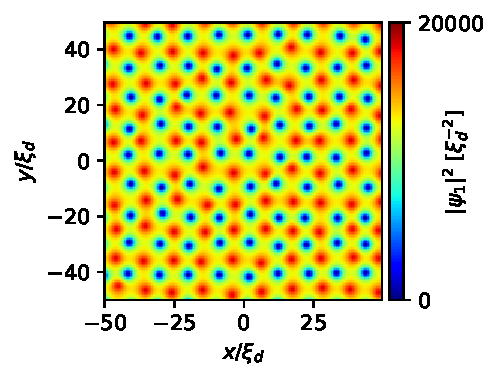
\includegraphics{gfx/ch-twoCompDynamics/init_state.pdf}
    \caption[Initial state of a two-component system filled with half-quantum
    vortices]
    {Density of \(\psi_1 \) component in a \(100\xi_d\times100\xi_d\)
        subregion of the initial state after imaginary time propagation.
        We see the HQVs in this component by the density depletion.
        The density peaks correspond to the location of HQV cores in the other
        component, which have been filled by atoms in this
        component.\label{fig:initial-vortex-state}}
\end{figure}
Previous work has shown that clustering of vortices can lead to anomalously
slow coarsening dynamics~\cite{Karl2017} and thus constructing the initial
state this way ensures that there is no clustering of like-signed vortices.
From this initial state, the system evolves according to
Eq.~\eqref{eq: dimensionless-two-comp-GPEs}.
Two HQVs in the same component with opposite winding can annihilate, leading to
a decay of the total vortex number within the system.

\section{Spatial aspects of half-quantum vortex decay}
We begin our investigations by considering the spatial aspects of the
relaxation dynamics.
Firstly, we wish to investigate how \(\gamma \) affects the HQVs within our
systems.
\begin{figure}
    \centering
    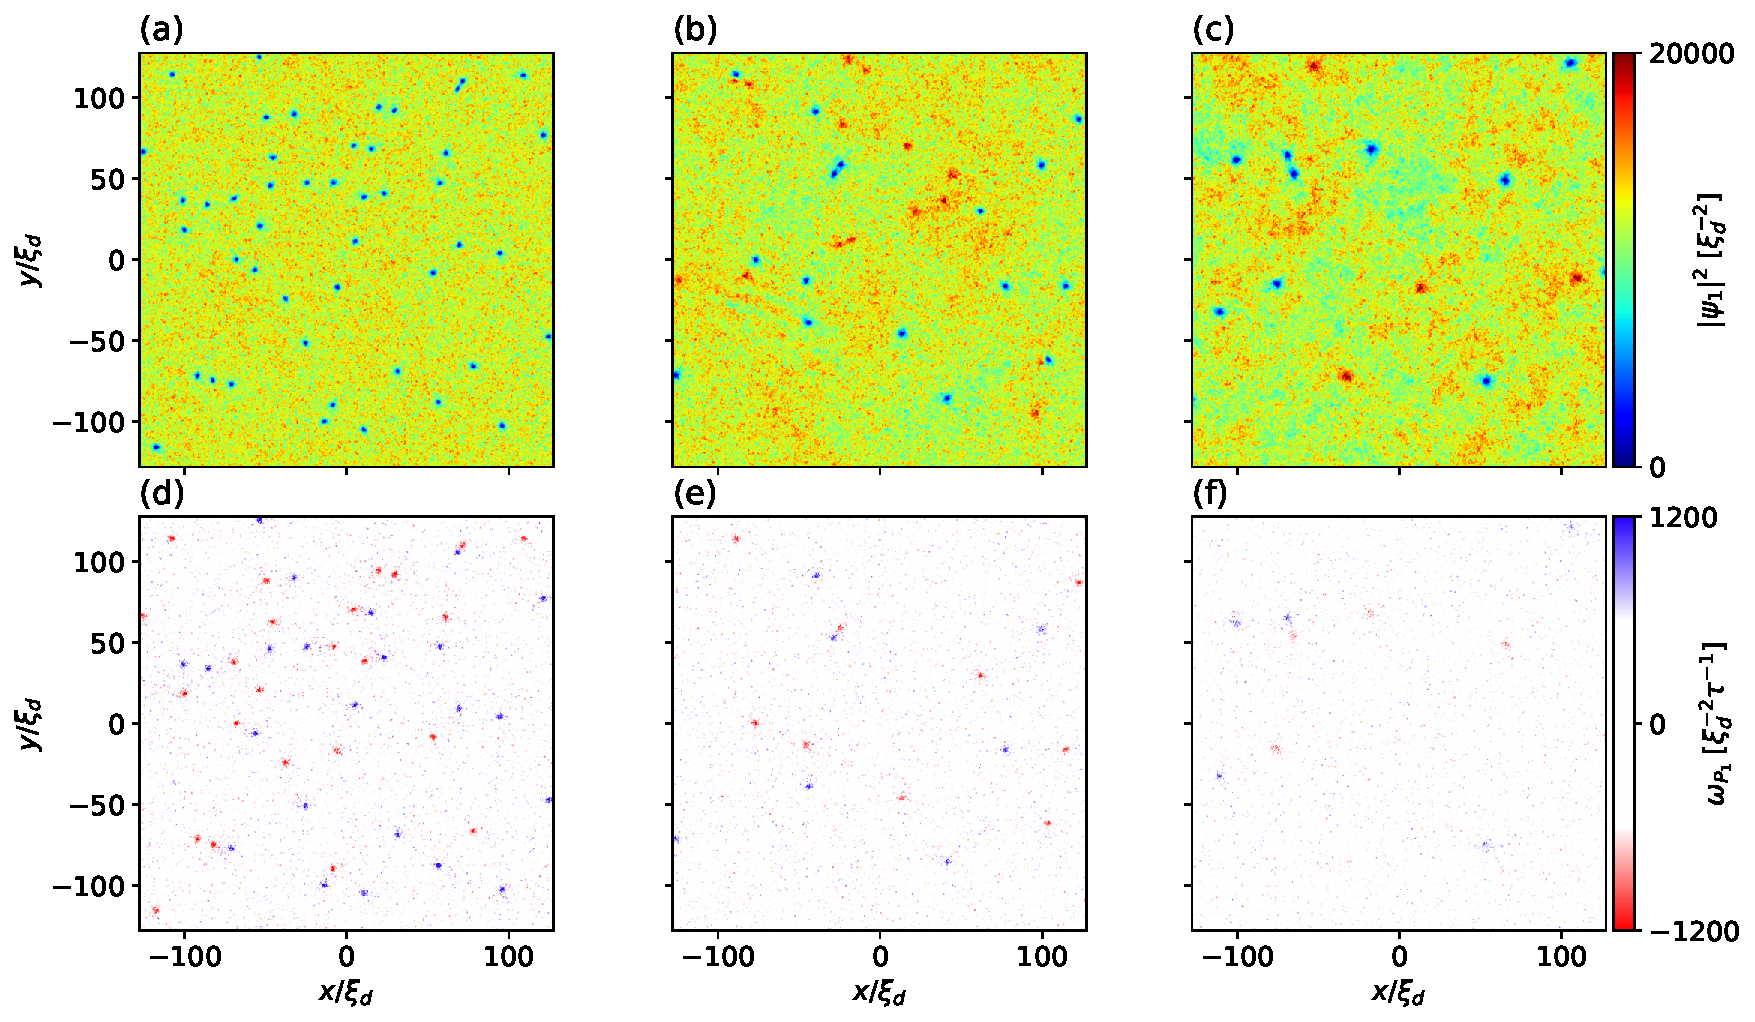
\includegraphics[width=\textwidth]{gfx/ch-twoCompDynamics/densVort.pdf}
    \caption[Density and pseudo-vorticity of a system during relaxation dynamics
    for various ratios of inter- to intra-species interaction.]
    {\label{fig:density-pseudo-vort}Density (a) {--} (c) and pseudo-vorticity
        (d) {--} (f) of the \(\psi_1 \) component in a
        \(256\xi_d \times 256\xi_d\) subregion at a time
        \(t/\tau=2.5\times 10^4\xi_d^2\) for \(\gamma=0.1\) (left),
        \(\gamma=0.6\) (middle), and \(\gamma=0.8\) (right).
        The density depletions correspond to HQVs in this component.
        For \(\gamma \gtrsim 0.6\), density peaks reveal the locations of HQVs
        with the phase singularity in the other component, where the vortex
        cores have filled with atoms in this component.
        Vortices with positive (blue) and negative (red) circulation are
        identifiable in the pseudo-vorticity field.}
\end{figure}
Fig.~\ref{fig:density-pseudo-vort} shows the density field of the \(\psi_1 \)
component for \(\gamma = 0.1, 0.6, 0.8\).
One sees that as \(\gamma \) increases, the core size (i.e., the radial size of
the density depletion) also increases.
From Eq.~\eqref{eq:healing-lengths} we see that the size of the HQV core is
dependent on \(\gamma \), where \(\xi_s \rightarrow \xi_d\) as
\(\gamma \rightarrow 0\).
The healing lengths can explain why, for \(\gamma \geq 0.6\), bright density
peaks also appear within the \(\psi_1 \) field.
For small \(\gamma \), the density and spin healing lengths become comparable,
\(\xi_d \sim \xi_s\).
However, an increasing \(\gamma \) implies a larger spin healing length.
Consequently, atoms of the other component will fill the vortex core as the
resulting lowering of the kinetic energy offsets the cost of interaction energy.
This results in the expansion of the vortex cores to the size of the spin
healing length.
Hence, bright density peaks in Fig.~\ref{fig:density-pseudo-vort} correspond to
atoms in the \(\psi_1 \) component that have filled the core of an HQV in the
\(\psi_2\) component.

To locate the HQVs in the system, we make use of the
pseudo-vorticity~\cite{Villois2016}, given as:
\begin{equation}
    \omega_\mathrm{p_j} = \frac{1}{2}\nabla \times {(n\vb{v})}_j,
\end{equation}
where \({(n\vb{v})}_j\) is the mass current of component \(j=1, 2\) defined as
in Eq.~\eqref{eq: two-comp-mass-current}.
The pseudo-vorticity has the unique property of remaining regular and non-zero
within the vortex cores, and, on length scales greater than the spin healing
length away from a vortex core, quickly relaxes to zero.
Therefore, this becomes a useful tool to identify where vortices are in the
system by checking for regions of non-zero pseudo-vorticity.
Fig.~\ref{fig:density-pseudo-vort} (d) {--} (f) shows the pseudo-vorticity for
the same systems in (a) {--} (c).
We see that non-zero regions of pseudo-vorticity are in alignment with the
density depletions, confirming the cores of vortices.
Additionally, the sign of the pseudo-vorticity also determines the charge of
the vortex, where positive pseudo-vorticity corresponds to a vortex with a
positive charge and vice versa.

\subsection{Investigating the kinetic energy spectrum}
A useful property to investigate in turbulent systems is the kinetic energy
spectrum, which provides useful insights into the spatial aspects of the
relaxation dynamics.
We start with the kinetic energy of the two-component system which is written
in terms of the density \(n_j\) and velocity \(\vb{v}_j\) of the \(j\)-th
component as
\begin{align}
    E_\mathrm{kin} = \int \left(|\nabla\sqrt{n_1}|^2
    + |\nabla\sqrt{n_2}|^2\right) \, \dd^2\vb{r} 
    + \frac{1}{4}\int \left(|\sqrt{n_1}\vb{v}_1|^2
    + |\sqrt{n_2}\vb{v}_2|^2\right) \, \dd^2\vb{r}.
\end{align}
The kinetic energy can be further decomposed into quantum pressure
(\( E^q\)) and classical velocity (\(E^v\)) contributions:
\begin{align}
    E^v = \frac{1}{4}\int \left(|\sqrt{n_1}\vb{v}_1|^2
    + |\sqrt{n_2}\vb{v}_2|^2\right) \, \dd^2\vb{r},
\end{align}
\begin{align}
    E^q = \int \left(|\nabla\sqrt{n_1}|^2
    + |\nabla\sqrt{n_2}|^2\right) \, \dd^2\vb{r}.
\end{align}
To extract energy spectra from these contributions we define the generalized
velocities for the incompressible (i), compressible (c), and quantum pressure
(q) parts as~\cite{Schmied2019}
\begin{align}
    \vb{w}^{i, c} &= \sqrt{n_1}\vb{v}_1^{i, c} + \sqrt{n_2}\vb{v}_2^{i, c} \\
    \vb{w}^q      &= 2 (\nabla \sqrt{n_1} + \nabla \sqrt{n_2}).
\end{align}
Here, the incompressible and compressible parts of the velocity field,
\(\vb{v}\), are extracted from a Helmholtz decomposition which splits the
velocity into a divergence-free incompressible part,
\(\nabla \cdot \vb{v}^i = 0\), and an irrotational, compressible part,
\(\nabla \times \vb{v}^c=\vb{0}\).
Hence, in Fourier space, the kinetic energy spectrum can be calculated by
taking the Fourier transform of the generalized velocities and integrating over
the \(k\)-space angle as
\begin{align}
    E^\delta(k) = \frac{1}{4} \int_{0}^{2\pi}
    |\tilde{\vb{w}}^\delta(\vb{k})|^2 \, \dd\Omega_k
    \qquad (\delta = i, c, q),
\end{align}
where \(\tilde{\vb{w}}^\delta \) denotes the Fourier transform of the
generalised velocity \(\vb{w}^\delta \) for wave number \(k=|\vb{k}|\).
The total kinetic energy is then given by the sum of each contribution,
integrated over all \(k\)
\begin{align}
    E_\mathrm{kin} = \sum_\delta \int E^\delta (k) \, \dd k
    \qquad (\delta = i, c, q).
\end{align}
The occupation numbers of each contribution are extracted as
\begin{align}
    n^\delta(k) = k^{-2}E^\delta(k) \qquad (\delta = i, c, q).
\end{align}
Finally, the total occupation number of the system is given as
\begin{align}
    n(k) = \int_{0}^{2\pi} \left[\tilde{\psi}_1^*(k)\tilde{\psi}_1(k)
    + \tilde{\psi}_2^*(k)\tilde{\psi}_2(k)\right] \, \dd \Omega_k.
\end{align}

\begin{figure}[t!]
    \centering
    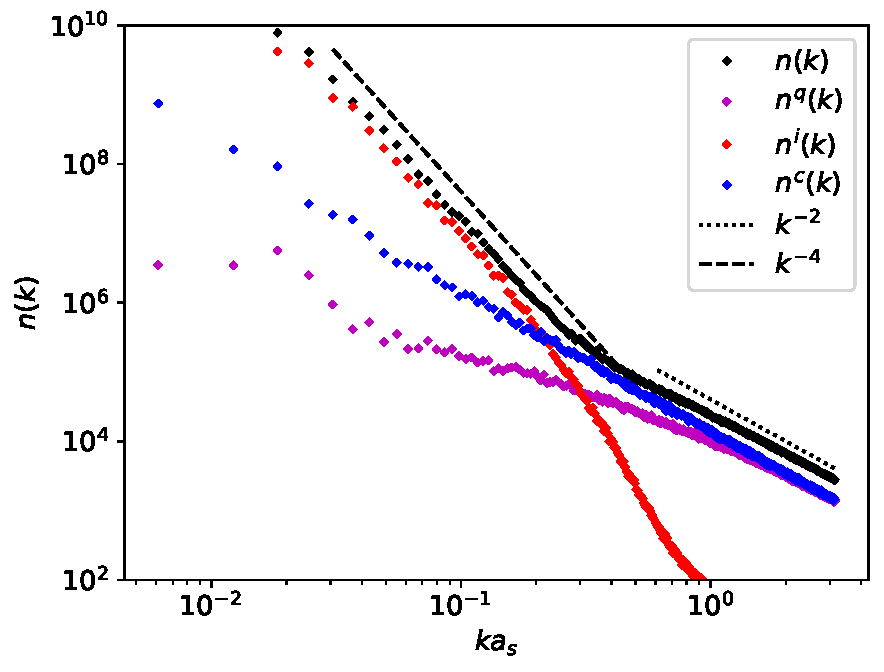
\includegraphics[scale=0.75]{gfx/ch-twoCompDynamics/spectra.pdf}
    \caption[Occupation numbers for quantum pressure, incompressible and
    compressible contributions for a two-component system during relaxation
    dynamics]
    {Occupation numbers for the quantum pressure (purple),
        incompressible (red diamonds), and compressible (blue)
        contributions for \(\gamma=0.6\).
        The total occupation number (black) is obtained from the sum of
        each contribution.
        The total occupation number has two distinct scaling: a \(k^{-2}\)
        (dotted line) in the ultraviolet region, and a \(k^{-4}\) scaling
        (dashed line) in the infrared.\label{fig:kinetic-energy-spectra}}
\end{figure}
We plot the occupation number for each energy contribution, as well as total
occupation number, at a late time for \(\gamma=0.6\) in
Fig.~\ref{fig:kinetic-energy-spectra}.
The total occupation number exhibits two different scaling: A \(k^{-4}\) in the
ultraviolet (UV), and \(k^{-2}\) in the infrared (IR).
The same scaling have been found in some 2D, turbulent, scalar BEC systems
containing scalar vortices~\cite{Nowak2012}.
The decomposition of the kinetic energy into its respective contributions
allows us to see that the incompressible contribution dominates the spectrum
in the IR region, and is therefore responsible for the transition to the
\(k^{-4}\) scaling.
This incompressible contribution is directly associated with the vortices in
the system, as vortices are the only excitations that can arise in an
incompressible, irrotational superfluid~\cite{Pethick2008,Barenghi2016}.
Similarly, we see it is both the compressible and quantum pressure contributions
that dominate in the UV region, facilitating the transition to the \(k^{-2}\)
scaling, which is characteristic of weak-wave-turbulence~\cite{Zakharov1992,
Nazarenko2011, Newell2011}.
This scaling of the kinetic energy was observed throughout all values of
\(\gamma \) tested, indicating that it is quantitatively insensitive to
variations in \(\gamma \).
The investigation into the kinetic energy spectrum thus reveals that \(\gamma \)
has negligible effects on the spatial aspects of the relaxation dynamics.
In addition, it shows that, despite containing a different type of vortex, the
dynamics follow quantitatively similar behaviour to some turbulent scalar BEC
systems containing scalar vortices~\cite{Nowak2012}.

\section{Temporal aspects of half-quantum vortex decay}
\subsection{Growth of correlation lengths}
To measure the temporal aspect of the relaxation dynamics, we will consider
correlation functions.
Since our pseudospin-1/2 order parameter is composed of a mass part and a spin
part [c.f. Eq.~\eqref{eq: Theta-Phi}], it is natural to then construct both a
mass and spin correlation function.
To begin, we need to identify appropriate quantities that serve as order
parameters for our system.
Motivated by the form of the EPP phase in spinor BECs, one such quantity is
the planar tensor~\cite{Symes2017}
\begin{equation}
    \mathsf{Q} = \mqty(Q_{xx} & Q_{xy} \\ Q_{xy} & -Q_{xx}),
\end{equation}
where \(Q_{xx} = \mathrm{Re}(\psi_1^*\psi_2)\) and
\(Q_{xy} = \mathrm{Im}(\psi_1^*\psi_2)\).
The eigenvalues of \(\mathsf{Q}\) are given by
\( \left\{-\frac{1}{2}|\alpha|, \frac{1}{2}|\alpha|\right\} \), where
\(\alpha=-2\psi_1\psi_2\).
If we consider the general wave function defined in
Eq.~\eqref{eq: pseudospin-1/2-wavefunction}, then evaluating \(\mathsf{Q}\) and
\(\alpha \) gives
\begin{equation}
    Q_{xx} = |\psi_1||\psi_2|\cos({2\Phi}), \qquad
    Q_{xy} = -|\psi_1||\psi_2|\sin({2\Phi}),
\end{equation}
\begin{equation}
    \alpha = -2|\psi_1||\psi_2|e^{2i\Theta}.
\end{equation}
This shows that \(\mathsf{Q}\) is dependent on the phase of the spin,
\( \Phi \), whereas \(\alpha \) is dependent upon the global phase,
\( \Theta \).

Armed with these quantities, we can then construct correlation functions related
to the mass and spin parts of our pseudo-spinor order parameter.
These are defined, respectively, as
\begin{equation}
    G_\Theta = \frac{1}{n^2}\langle \alpha^*(\vb{0})\alpha(\vb{r}) \rangle,
\end{equation}
\begin{equation}
    G_\Phi(\vb{r}, t) =
    \frac{2}{n^2}\mathrm{Tr}
    [\langle \mathsf{Q}(\vb{0})\mathsf{Q}(\vb{r})\rangle],
\end{equation}
where \( \langle \cdot \rangle \) denotes ensemble averaging.
By exploiting the fact that our system is homogeneous, we can replace ensemble
averages with spatial averages.
To obtain the 1D spectrum, we perform an angular integration in k-space.
The spin correlation function is then computed as
\begin{equation}
    G_\Phi(r, t) = \int d\Omega_k \int \frac{d^2\vb{r}^\prime}{L^2}
    \frac{2}{n^2}\text{Tr}
    [\langle \mathsf{Q}(\vb{r}^\prime)\mathsf{Q}(\vb{r}^\prime+\vb{r})\rangle],
\end{equation}
where \(\int d\Omega_k\) denotes integration over the k-space angle, whilst
\(\int d^2\vb{r}'/L^2\) is spatial averaging.
We perform the same averaging for the mass correlation function.

\begin{figure}
    \centering
    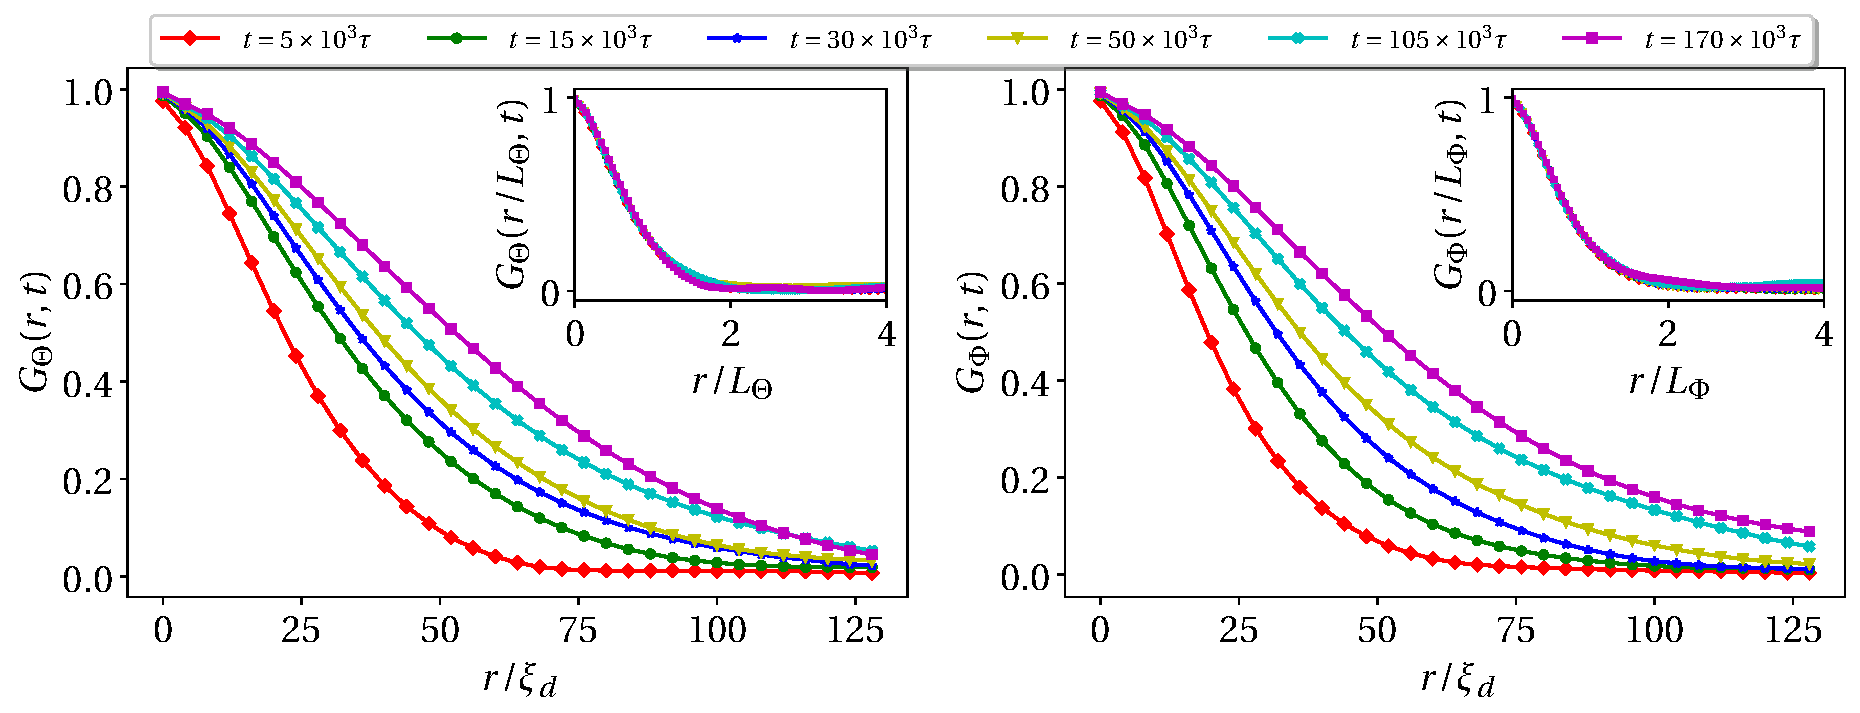
\includegraphics[width=\textwidth]{
        gfx/ch-twoCompDynamics/correlation_functions.pdf}
    \caption[Mass and spin correlation functions associated with half-quantum
    vortex relaxation dynamics]{\label{fig: correlation-functions}Correlation
    functions for the mass (left) and spin (right) parts of a two-component
    system as functions of time for \(\gamma=0.6\).
    As time increases the correlation functions decay over a larger range,
    indicating long-rang ordering within the system.
    Insets: Collapse of the mass (left) and spin (right) correlation functions
    when scaled by the appropriate correlation length.}
\end{figure}
Fig.~\ref{fig: correlation-functions} shows both correlation functions for
\(\gamma=0.6\) for various times through the simulation.
We see that as time increases, the correlation functions extend over larger
distances which indicates that the respective domains are growing over time,
showing long-range order is being established.
From these correlation functions, we may extract a correlation length,
\(L_\delta \) with \(\delta \in \{\Theta, \Phi \} \), that enables us to
determine a length scale over which the correlation function decays.
We take the correlation length to be the value at which the corresponding
correlation function decays to a quarter of its value at
\(r=0\): \(G_\delta(L_\delta, t) = \frac{1}{4}G_\delta(0, t)\).
Using the correlation length, we can determine whether the correlation functions
exhibit dynamical scaling, which implies the form of the functions remains
self-similar at different times throughout the simulation.
This means the function collapses to a universal, time-independent function
when scaled by the correlation length: \(H_\delta(r) = G(r/L_\delta(t), t)\).
The insets of Fig.~\ref{fig: correlation-functions} show the scaling of the
correlation functions when scaled by the respective correlation length.
This confirms that the correlation functions within our system do exhibit
dynamical scaling.

\begin{figure}
    \centering
    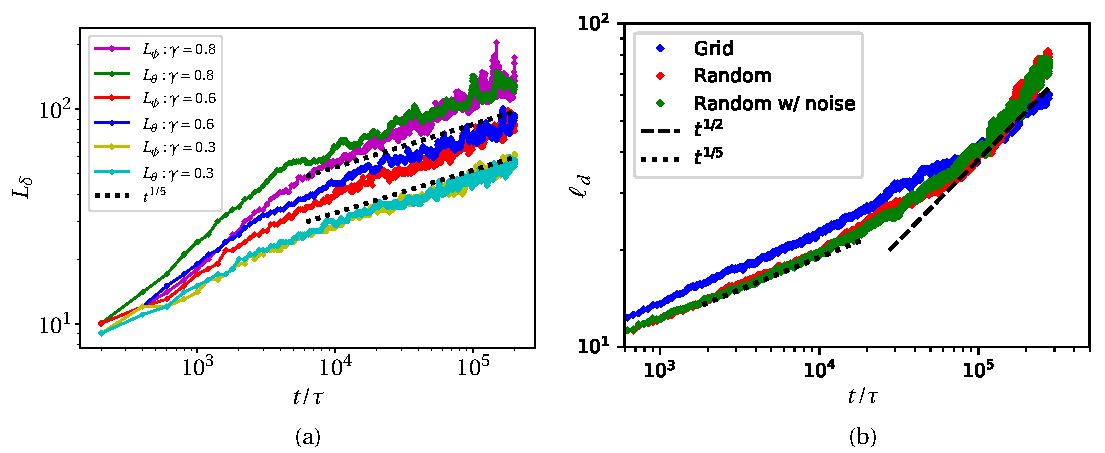
\includegraphics[width=\textwidth]{
        gfx/ch-twoCompDynamics/two-component-correlation-lengths.pdf}
    \caption[Mass and spin correlation lengths associated with half-quantum
    vortex relaxation dynamics, in addition to inter-vortex spacing in a scalar
    system]{\label{fig: correlation-lengths} (a): Mass and spin correlation
    lengths as a function of time for \(\gamma=0.3,0.6, 0.8\).
    For early-time dynamics, a larger \(\gamma \) is associated with a faster
    growth of the correlation length.
    At late times, however, all correlation lengths tend to a universal
    \(t^{1/5}\) scaling.
    (b): Inter-vortex spacing, \(\ell_d\), as a function of time for scalar
    systems prepared using different initial conditions.
    Grid corresponds to a grid of vortices, similar to the setup in (a), random
    (with noise) corresponds to a random distribution of vortices where each
    position is drawn from a uniform distribution (with numerical noise added
    to the initial state).
    For early-time dynamics the inter-vortex spacing follows a
    \(t^{1/5}\) for each initial state.
    At late times, this scaling transition to \(t^{1/2}\), which is typically
    observed in scalar vortex relaxation dynamics~\cite{Nowak2012}.
    }
\end{figure}
Fig.~\ref{fig: correlation-lengths} shows the correlation lengths for
\(\gamma=0.3\), \(\gamma=0.6\), and \(\gamma=0.8\) as functions of time.
We see that at late times in the evolution, all correlation lengths tend to a
universal \(t^{1/5}\) scaling.
However, the early-time dynamics are remarkably different for the various
\(\gamma \).
As \(\gamma \) increases, there is a faster growth of the correlation lengths at
early times, which signifies the correlation length being \(\gamma \)-dependent.
We investigate this behaviour by considering the total vortex number of
the system as a function of time.
We can then extract the mean distance between the vortices as
\(\ell_d=1/\sqrt{N_\mathrm{vort}}\), where \(N_\mathrm{vort}\) is the total
number of vortices in the two components.
In a scalar BEC containing an initially large number of vortices, it has been
observed that \(\ell_d \sim t^\beta \)~\cite{Karl2017}, where \(\beta \)
characterizes the annihilation rate of vortices.
In particular, there were two distinct \(\beta \) observed: Firstly, a
\(\beta=1/5\) scaling after some short period of evolution.
This scaling is included in Fig.~\ref{fig: correlation-lengths}a as a
comparison.
Secondly, after a much longer period of evolution, a \(\beta=1/2\) scaling
emerges.
This second scaling can be delayed if the initial vortex distribution is
highly clustered~\cite{Karl2017}.

Fig.~\ref{fig: correlation-lengths}b is a reproduction of both the early- and
late-time scaling of the mean vortex distance, \(\ell_d\), for a scalar system
using the parameters of~\cite{Karl2017}.
We consider three initial conditions: Firstly, we constructed a grid of vortices
analogous to our two-component system (see
Sec.~\ref{subsec: two-comp-numerical-setup}).
Secondly, we considered a random distribution of vortices; one with noise
added to the energy spectrum, and one without.
We see that at early and intermediate times, there is a clear \(t^{1/5}\)
scaling in all the initial states tested.
Furthermore, at late times we recover the \(t^{1/2}\) scaling for all initial
states.
This indicates the scaling is robust and insensitive to the initial conditions.

\subsection{Vortex decay rate}
Motivated by this previous work in scalar BECs~\cite{Karl2017}, we conduct a
similar analysis on our two-component system containing HQVs, and determine how
\(\gamma \) affects the vortex decay rate.
In particular, we consider the early-time evolution in which
Fig.~\ref{fig: correlation-lengths}a suggests interesting dynamics.
\begin{figure}
    \centering
    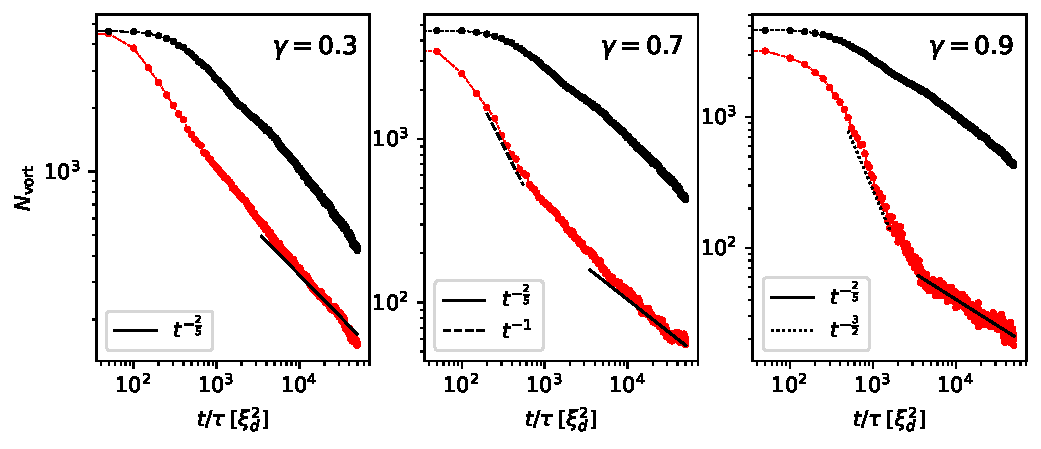
\includegraphics[width=\textwidth]{gfx/ch-twoCompDynamics/vortex_number.pdf}
    \caption[Vortex decay as a function of time for a system of half-quantum
    vortices for different ratios of inter- to intra-species interaction]
    {\label{fig: vortex-number}Total vortex number as a function of time for
        \(\gamma=0.3,0.7,0.9\) (red circles).
        Larger \(\gamma \) leads to a faster decay rate of vortices at
        early times due to the rapid annihilation of opposite-signed vortices
        within the same component.
        Despite vastly different early-time dynamics, the vortex decay rates
        tend to a universal \(t^{-2/5}\) at late times.
        For comparison the vortex decay rate of a scalar system is shown
        (black circles).
        This system is set up using the grid method as defined in
        Sec.~\ref{subsec: two-comp-numerical-setup}, with \(48^2\) vortices in
        total.
        Note that the black line is multiplied by two to have it be the same
        total vortex number as the two-component system.
    }
\end{figure}
The variation of the total vortex number with time is plotted in
Fig.~\ref{fig: vortex-number} for \(\gamma=0.3\), \(\gamma=0.7\), and
\(\gamma=0.9\).
We see that for \(\gamma=0.3\), the vortex decay rate is mostly consistent
throughout the evolution, which tends to a \(t^{-2/5}\)
(\(\ell_d \sim t^{1/5}\)) scaling at later times.
More interesting dynamics are revealed for \(\gamma=0.7, 0.9\) where two
different scaling regimes emerge at early times
(\(2.5\times10^2\xi_d^2 \lesssim t/\tau \lesssim 2.5\times10^3\xi_d^2\)) with
\(N_\mathrm{vort} \sim t^{-1}\) for \(\gamma=0.7\) and
\(N_\mathrm{vort} \sim t^{-3/2}\) for \(\gamma=0.9\).
After the initial differing early-time dynamics, the systems then tend to a
universal \(t^{-2/5}\) scaling, which corresponds to \(\ell_d\sim t^{1/5}\)
similar to the scalar BEC simulation shown.
These results show a better fit to the theoretical \(t^{1/5}\) scaling than
indicated by the correlation lengths shown in
Fig.~\ref{fig: correlation-lengths}.
This further suggests that \(L_{\Phi,\Theta}\) differs slightly from \(\ell_d\),
even though the growth of the correlation lengths is driven by vortex
annihilation.
Fig.~\ref{fig: vortex-number} only extends up to \(t/\tau=5\times 10^4\xi_d^2\),
and we expect to see a universal transition to
\(N_\mathrm{vort}\sim t^{-1}\) (\(\ell_d\sim t^{1/2}\)) at much later times for
sufficiently small \(\gamma \).
For large \(\gamma \), due to the rapid annihilation of vortices at early times,
there may not be enough vortices left within the system to facilitate the
transition to the \(N_\mathrm{vort} \sim t^{-1}\) regime.

We wish to investigate further the effect of \(\gamma \) on the initial decay
rate of the vortices.
We can model the vortex decay rate as a simple kinetic-like equation of the form
\begin{equation}
    \pdv{N_\mathrm{vort}}{t} \sim N_\mathrm{vort}^\eta,
\end{equation}
where \(\eta > 1\).
The form of this equation states that the decay rate of the vortices is
dependent on the total number of vortices facilitating the annihilation.
Using this simple model, we can extract a scaling for the total vortex
number as
\begin{equation}
    N_\mathrm{vort} \sim t^{-2/z},
    \label{eq:vortex-number-scaling}
\end{equation}
where \(z=-2(1-\eta)\).
An exponent of \(z=2\) corresponds to a two-body collision process, in which
only two vortices are required to annihilate.
On the contrary, an exponent of \(z=5\) corresponds to a three-body collision
process, where three vortices are necessary to facilitate annihilation.
\begin{figure}[t!]
    \centering
    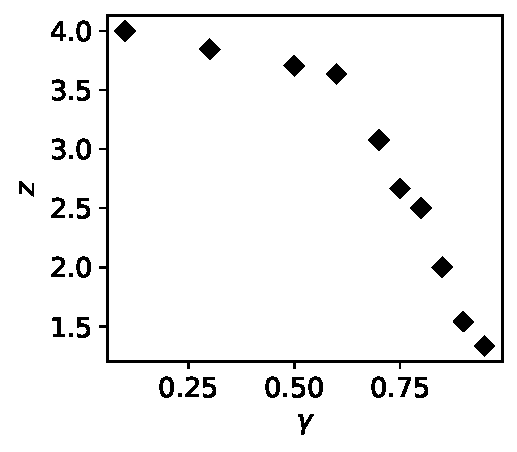
\includegraphics[width=0.85\textwidth]{
        gfx/ch-twoCompDynamics/gamma_vs_expo.pdf}
    \caption[Critical exponent of the vortex decay scaling as a function of the
    ratio of inter- to intra-species interaction]
    {\label{fig: exponent-vs-gamma}The exponent \( z \) in
        Eq.~\eqref{eq:vortex-number-scaling} as a function of \(\gamma \).
        Here, \(z\) is calculated in the region \(2.5 \times 10^2\xi_d^2 <
        t/\tau < 2.5\times10^3\xi_d^2\), where early-time dynamics take place.
        We see that after \(\gamma \gtrsim 0.6\) a rapid decrease of the
        exponent occurs, signalling a rapid change in vortex dynamics.}
\end{figure}
Fig.~\ref{fig: exponent-vs-gamma} shows the exponent, \( z \), as a function of
\(\gamma \) where \( z \) is extracted within the time interval
\(2.5 \times 10^2\xi_d^2 < t/\tau < 2.5\times10^3\xi_d^2\).
We see a rapid decrease of the exponent after \(\gamma \gtrsim 0.6\), in which
Fig.~\ref{fig: vortex-number} shows the rapid annihilation of vortices is
prevalent.
The decrease of the exponent in our simulations signals an additional vortex
interaction mechanism not present in scalar BEC systems.

Numerous studies have been conducted to try to understand the inter-vortex
forces between HQVs in two-component systems~\cite{Eto2011, Kasamatsu2016}.
In particular, Kasamatsu \textit{et al.}~\cite{Kasamatsu2016} tried to derive a
point vortex model to explain the dynamics shown in
Fig.~\ref{fig: exponent-vs-gamma}, but found that the model failed to accurately
predict the resulting vortex dynamics.
They conducted simple tests involving a dipole of HQVs in which they found that
an increase in \(\gamma \) dramatically changes the motion of the dipole.
For \(\gamma>=0.6\), it was found that the individual vortices move together and
undergo annihilation.
For weaker \(\gamma \), the two vortices move in parallel, similar to
the behaviour observed for dipoles consisting of scalar \(\mathrm{U}(1)\)
vortices.
The strength of \(\gamma \) also determines the rate at which the vortices
annihilate (see Fig. 11 of Ref.~\cite{Kasamatsu2016}).

\section{Conclusions}
In this chapter we have investigated the relaxation dynamics of HQVs in a
two-dimensional, two-component BEC\@.
After detailing the numerical set up, we first investigated the spatial aspects
of the relaxation dynamics.
In particular, we investigated the kinetic energy spectrum by splitting it
into incompressible, compressible, and quantum pressure parts.
We found that the kinetic energy spectrum exhibits two different scaling in the
infrared and ultraviolet regions.
The former had a scaling of \(k^{-2}\), whilst the latter had \(k^{-4}\).
The splitting of the spectrum into its constituent parts revealed that the
transition to the \(k^{-2}\) scaling was due to the incompressible component,
whilst the \(k^{-4}\) arose due to the compressible component.
Similar scaling has been observed in scalar BEC systems containing scalar
vortices~\cite{Nowak2012}.
This shows that, despite being an entirely different class of vortex, relaxation
dynamics of HQVs exhibit similar spatial aspects to those observed in scalar
systems with scalar vortices

After considering the spatial aspects, we then considered the temporal aspects
of the relaxation dynamics.
We started with investigating the correlation functions, for which we
constructed both a mass and spin part.
It was revealed that the correlation functions extended over larger regions as
time increased, which indicates long-range order within our systems.
We also showed our system exhibits dynamical scaling, by showing that the
correlation functions collapsed to a universal, time-independent function when
scaled by the appropriate correlation length.
Investigations into these correlation lengths suggested anomalous early-time
dynamics was taking part.
It was revealed that the correlation lengths had a faster initial growth for
larger \(\gamma \), but at late times all correlation lengths scaled as
\(t^{1/5}\).

Motivated by the previous scalar BEC work in~\cite{Karl2017}, we investigated
the decay rate of the vortices.
We showed that for sufficiently high \(\gamma \gtrsim 0.6\) the vortices had an
increasingly steeper decay rate at early times, which then tended to a universal
\(t^{-2/5}\) at late times in all \(\gamma \) tested.
We tested this theory further by modelling the vortex decay rate as a simple
kinetic-like equation, for which we then manually extracted the scaling of
the total vortex number.
Plotting the exponent of the scaling against \(\gamma \) confirmed that after
\(\gamma \sim 0.6\) there is a rapid increase the exponent, and therefore the
decay rate of the vortices.